% documentclass options:
\documentclass[11pt,
  a4paper,
  parskip=half, % This is some extra vertical space between paragraphs, the suggestion is 2cm which is really ugly, so we use what koma script gives us
  % you can also set it to full for even more space. But there is a bad tex style decision: parskip also changes the spacing between listitems such as
  % enumerate and itemize. For this purpose we include the enumitem package and set itemsep=.5em, of course you can change this
  BCOR=10mm, % BCOR is binding correction
  english,
  % if you'd rather have a one sided thesis, add `oneside' to the documentclass
  % onside,
  % ngerman is needed for hyphenation if the thesis contains parts written in German, switch order with english if you write mainly in English.
  % Remember to change order in the babel package (below) as well.
  % Last language is the preferred one.
  ngerman]{scrbook}
\usepackage[english]{babel} % If you write mainly in English change order to ngerman, english. Also change that in the documentclass options above.
% Include of titling must happen before \title etc.
% that's why it's not in setup.tex
\usepackage{titling}
\title{How does a token based order compare to the asynchron order in multi-agent plan executions?}
\author{Felicitas Ritter}

% Change to your first examiner
% The ~ enables non sentence spacing after a period
\newcommand{\firstexaminer}{Prof.~Dr.~B. Nebel}
% Change to your second examiner, some undergraduate studies don't have a second examiner
% in this case just comment out the following line
%\newcommand{\secondexaminer}{Prof.~Dr.~Wile E. Coyote}
% Change to your adivers
\newcommand{\advisers}{Dr. Robert Mattmüller, Thorsten Engesser}

% include all packages and define commands in setup.tex

%------------------------------------------------------------------------------
%       package includes
%------------------------------------------------------------------------------
    % font encoding is set up for pdflatex, for other environments see
    % http://tex.stackexchange.com/questions/44694/fontenc-vs-inputenc
    \usepackage[T1]{fontenc}  % 8-bit fonts, improves handling of hyphenations
    \usepackage[utf8x]{inputenc}
    % provides `old' commands for table of contents. Eases the ability to switch
    % between book and scrbook
    \usepackage{scrhack}


    % ------------------- layout, default -------------------
    % adjust the style of float's captions, separated from text to improve readabilty
    \usepackage[labelfont=bf, labelsep=colon, format=hang, textfont=singlespacing]{caption}
    % With format = hang your caption will look like this:
    % Figure 1: Lorem ipsum dolor sit amet,
    %           consectetuer adipiscing elit.
    %           Ut purus elit, vestibulum
    % If you instead want
    % Figure 1: Lorem ipsum dolor sit amet,
    % consectetuer adipiscing elit. Ut purus
    % elit, vestibulum
    % change to format=plain
    \usepackage{chngcntr}  % continuous numbering of figures/tables over chapters
    \counterwithout{equation}{chapter}
    \counterwithout{figure}{chapter}
    \counterwithout{table}{chapter}

    % Uncomment the following line if you switch from scrbook to book
    % and comment the setkomafont line
    %\usepackage{titlesec}  % remove "Chapter" from the chapter title
    %\titleformat{\chapter}[hang]{\bfseries\huge}{\thechapter}{2pc}{\huge}
    \setkomafont{chapter}{\normalfont\bfseries\huge}

    \usepackage{setspace}  % Line spacing
    \onehalfspacing
    % \doublespacing  % uncomment for double spacing, e.g. for annotations in correction

    % ------------------- functional, default-------------------
    \usepackage[dvipsnames]{xcolor}  % more colors
    \usepackage{array}  % custom format per column in table - needed on the title page
    \usepackage{graphicx}  % include graphics
    \usepackage{subfig}  % divide figure, e.g. 1(a), 1(b)...
    \usepackage{amsmath}  % |
    \usepackage{amsthm}   % | math, bmatrix etc
    \usepackage{ amssymb }
    \usepackage{amsfonts} % |
    \usepackage{calc}  % calculate within LaTeX
    \usepackage[unicode=true,bookmarks=true,bookmarksnumbered=true,
                bookmarksopen=true,bookmarksopenlevel=1,breaklinks=false,
                pdfborder={0 0 0},backref=false,colorlinks=false]{hyperref}
    \usepackage{etoolbox} % if-else commands


    %==========================================
    % You might not need the following packages, I only included them as they
    % are needed for the example floats
    % ------------------- functional, custom -------------------
    \usepackage{algorithm,algpseudocode}
    \usepackage{bm}  % bold greek variables (boldmath)
    \usepackage{tikz}
    \usetikzlibrary{positioning}  % use: above left of, etc

    % required for the ToDo list
    \usepackage{ifthen}

    % Improves general appearance of the text
    \usepackage[protrusion=true,expansion=true, kerning]{microtype}
    \usepackage{enumitem}
    % nicer font for pdf rendering
    \usepackage{lmodern}

    % For nicer looking tables
    \usepackage{booktabs}

    % usually you don't need this, just for demonstration of a longer caption
    \usepackage{lipsum}

    %for color in mathmode
    \usepackage{xcolor}

    % for wrapping text around figures
    \usepackage{wrapfig}

%------------------------------------------------------------------------------
%       (re)new commands / settings
%------------------------------------------------------------------------------
    % ----------------- referencing ----------------
    \newcommand{\secref}[1]{Section~\ref{#1}}
    \newcommand{\chapref}[1]{Chapter~\ref{#1}}
    \renewcommand{\eqref}[1]{Equation~(\ref{#1})}
    \newcommand{\figref}[1]{Figure~\ref{#1}}
    \newcommand{\tabref}[1]{Table~\ref{#1}}

    % ------------------- colors -------------------
    \definecolor{darkgreen}{rgb}{0.0, 0.5, 0.0}
    % Colors of the Albert Ludwigs University as in
    % https://www.zuv.uni-freiburg.de/service/cd/cd-manual/farbwelt
    \definecolor{UniBlue}{RGB}{0, 74, 153}
    \definecolor{UniRed}{RGB}{193, 0, 42}
    \definecolor{UniGrey}{RGB}{154, 155, 156}


    % ------------------- layout -------------------
    % prevents floating objects from being placed ahead of their section
    \let\mySection\section\renewcommand{\section}{\suppressfloats[t]\mySection}
    \let\mySubSection\subsection\renewcommand{\subsection}{\suppressfloats[t]\mySubSection}



    % ------------------- math formatting commands -------------------
    % define vectors to be bold instead of using an arrow
    \renewcommand{\vec}[1]{\mathbf{#1}}
    \newcommand{\mat}[1]{\mathbf{#1}}
    % tag equation with name
    \newcommand{\eqname}[1]{\tag*{#1}}
    % format propositions
    \newtheorem{theorem}{Proposition}


    % ------------------- pdf settings -------------------
    % ADAPT THIS
    \hypersetup{pdftitle={\thetitle},
                pdfauthor={\theauthor},
                pdfsubject={Undergraduate thesis at the Albert Ludwig University of Freiburg},
                pdfkeywords={deep learning, awesome algorithm,  undergraduate thesis},
                pdfpagelayout=OneColumn, pdfnewwindow=true, pdfstartview=XYZ, plainpages=false}


    %==========================================
    % You might not need the following commands, I only included them as they
    % are needed for the example floats

    % ------------------- Tikz styles -------------------
    \tikzset{>=latex}  % arrow style

    \tikzset{
    world/.style={circle, fill, inner sep=1.5pt, outer sep=3pt},
    desig/.style={circle, draw, inner sep=3pt, outer sep=3pt},
    anchor=base, baseline}

    \newcommand{\preeff}[2]{%
    \begin{tabular}{l}pre: #1\\eff: #2\end{tabular}%
    }


    % ------------------- algorithm ---------------------
    % Command to align comments in algorithm
    \newcommand{\alignedComment}[1]{\Comment{\parbox[t]{.35\linewidth}{#1}}}
    % define a foreach command in algorithms
    \algnewcommand\algorithmicforeach{\textbf{foreach}}
    \algdef{S}[FOR]{ForEach}[1]{\algorithmicforeach\ #1\ \algorithmicdo}

    % line spacing should be 1.5
    \renewcommand{\baselinestretch}{1.5}

    % set distance between items in a list, for more details see the
    % enumitem package: https://www.ctan.org/pkg/enumitem
    \setlist{itemsep=.5em}

    % use ra in your tables to increase the space between rows
    % 1.3 should be fine
    \newcommand{\ra}[1]{\renewcommand{\arraystretch}{#1}}

	% ToDo counters
	\usepackage{ifthen} %für whiledo-Schleife
	\newcounter{todos}
	\setcounter{todos}{0}
	\newcounter{extends}
	\setcounter{extends}{0}
	\newcounter{drafts}
	\setcounter{drafts}{0}

	% ------------------- marker commands -------------------
    % ToDo command
    \newcommand{\todo}[1]{\textbf{\textcolor{red}{(TODO: #1)}}\refstepcounter{todos}\label{todo \thetodos}}
	\newcommand{\extend}[1]{\textbf{\textcolor{darkgreen}{(EXTEND: #1)}}\refstepcounter{extends}\label{extend \theextends}}
	% Lighter color to note down quick drafts
	\newcommand{\draft}[1]{\textbf{\textcolor{NavyBlue}{(DRAFT: #1)}}\refstepcounter{drafts}\label{draft \thedrafts}}

	% microtype with lmodern, see https://tex.stackexchange.com/questions/75305/microtype-warning-with-lmodern-package-and-koma-script
	%\DeclareMicrotypeAlias{lmss}{cmr}


\begin{document}
    \pagestyle{empty} % no header and no page number
    % disable hyper links to remove warning "destination with same identifier"
    % this means within this section nothing can be referenced with a hyperlink
    \hypersetup{pageanchor=false}

    % enable/disable, depending on your chosen language
    
\begin{titlepage}
\begin{center}

\newcommand{\HorizontalLine}{\rule{\linewidth}{0.3mm}}

{\Large Bachelor Thesis}\\[1.3cm]


% _____________________________________________________________________________
\HorizontalLine \\[0.4cm]
% Write your title in a fancy way like this if you want to customize it, otherwise simply let tex do it for you
% \begin{spacing}{3}
%     {\huge \bfseries The Long, Long } \\
%     {\huge \bfseries Long Long} \\
%     {\huge \bfseries Title}\\
% \end{spacing}
{ \huge \bfseries \thetitle }
\HorizontalLine \\[1.5cm]
% _____________________________________________________________________________


{\Huge \theauthor} \\[2cm]


\begin{tabular}[hc]{>{\huge}l >{\huge}l}
  Examiner: & \firstexaminer \\[0.3cm]
  Advisers: & Dr. Robert Mattmüller, \\[0.3cm]
   & Thorsten Engesser \\[1.2cm]
\end{tabular}
\vfill  % move the following text to the bottom

\Large {
    Albert-Ludwigs-University Freiburg\\
    Faculty of Engineering\\
    Department of Computer Science\\
    Chair for Foundations of Artificial Intelligence\\[1cm]

    August 07\textsuperscript{th}, 2019\\
}
\end{center}
\end{titlepage}

\thispagestyle{empty}
% title page back
\ \vfill \ \\  % at least one space required before vfill
\
\textbf{Writing Period}            \smallskip{} \\
07.\,05.\,2019 -- 07.\,08.\,2019   \bigskip{} \\
\
\textbf{Examiner}                  \smallskip{} \\
\firstexaminer                     \bigskip{} \\
\
% If there is a second examiner include it
\ifdef{\secondexaminer}
	{
	% Include
	\textbf{Second Examiner}       \smallskip{} \\
	\secondexaminer                \bigskip{} \\
	\
	}
	{
	% No second examiner, ignore
	}
\textbf{Advisers}                  \smallskip{} \\
\advisers

    %\begin{titlepage}
\begin{center}

\newcommand{\HorizontalLine}{\rule{\linewidth}{0.3mm}}

{\Large Bachelor Thesis}\\[1.3cm]


% _____________________________________________________________________________
\HorizontalLine \\[0.4cm]
% Write yourtitle in a fancy way like this if you want to customize it, otherwise simply let tex do it for you
% \begin{spacing}{3}
%     {\huge \bfseries Der Lange, Lange } \\
%     {\huge \bfseries Lange Lange} \\
%     {\huge \bfseries Titel}\\
% \end{spacing}
{ \huge \bfseries \thetitle }
\HorizontalLine \\[1.5cm]
% _____________________________________________________________________________


{\Huge \theauthor} \\[2cm]


\begin{tabular}[hc]{>{\huge}l >{\huge}l}
  Gutachter: & \firstexaminer \\[0.3cm]
  Betreuer: & \advisers \\[1.2cm]
\end{tabular}
\vfill  % move the following text to the bottom

\Large {
    Albert-Ludwigs-Universität Freiburg\\
    Technische Fakultät\\
    Institut für Informatik\\
    Lehrstuhl für Thesis-Templates\\[1cm]

    3. April 2017
    \\
}
\end{center}
\end{titlepage}

\thispagestyle{empty}
% title page back
\ \vfill \ \\  % at least one space required before vfill
\
\textbf{Bearbeitungszeit}            \smallskip{} \\
05.\,07.\,2016 -- 05.\,10.\,2016   \bigskip{} \\
\
\textbf{Gutachter}                  \smallskip{} \\
\firstexaminer                      \bigskip{} \\
\
% If there is a second examiner include it
\ifdef{\secondexaminer}
	{
	% Include
	\textbf{Zweitgutachter}        \smallskip{} \\
	\secondexaminer                \bigskip{} \\
	\
	}
	{
	% No second examiner, ignore
	}
\textbf{Betreuer}                  \smallskip{} \\
\advisers


    \pagestyle{plain} % remove chapter name from top, page number at the bottom
    % use \pagestyle{headings} for having the chapter on top of the pages
    % if you wang a more fancy header use \usepackage[automark,headsepline]{scrlayer-scrpage}
    % and read about it in the KOMA script documentation, https://www.ctan.org/pkg/koma-script
    \frontmatter  % roman page numbers
    % official declaration from the examination office; to be sure double
% check the wording on their website
% (https://www.tf.uni-freiburg.de/studies/exams/thesis/thesis_formatting.html#erklaerung)

\chapter*{Declaration}

I hereby declare, that I am the sole author and composer of my thesis and that no other sources or learning aids, other than those listed, have been used. Furthermore, I declare that I have acknowledged the work of others by providing detailed references of said work.  \newline
I hereby also declare, that my Thesis has not been prepared for another examination
or assignment, either wholly or excerpts thereof.
\\[3\normalbaselineskip]
\begin{tabular}{p{\textwidth/2} l}
  \rule{\textwidth/3}{0.4pt}   &   \rule{\textwidth/3}{0.4pt} \\
  Place, Date                  &   Signature
\end{tabular}

    \chapter*{Abstract}

In this thesis, we are going to use epistemic planning for the decision making process in multi-agent planning with distributed knowledge. In multi-agent domains, the agents are independent with the actions of other agent causing changes not instigated by the agent. We have used dynamic epistemic logic to model tokens to avoid problems with deadlocks and infinite executions in implicit coordination.
Through tokens, an agent can decide the next active agent. It is possible to solve planning tasks with joint goals without the agents having to negotiate about and commit to a centralized joint policy at plan time. We then analyzed this model by solving infinite executions and deadlocks.

\chapter*{Zusammenfassung}

In dieser Arbeit werden wir epistemische Planung für den Entscheidungsprozess in der Multi-Agent Planung mit verteiltem Wissen verwenden. In Multi-Agenten-Domänen sind die Agenten unabhängig von den Aktionen anderer Agenten, die Änderungen verursachen, die nicht vom Agenten eingeleitet wurden.
Wir haben die dynamische epistemische Logik für die Modellierung von Tokens verwendet, um Probleme mit Deadlocks und infinite executions bei der impliziten Koordination zu vermeiden. Durch Tokens kann ein Agent den nächsten aktiven Agenten entscheiden. Es ist möglich, Planungsaufgaben mit gemeinsamen Zielen zu lösen, ohne dass die Akteure zur Planzeit über eine zentralisierte gemeinsame Strategie verhandeln und sich dazu verpflichten müssen. Wir haben dann dieses Modell evaluiert, indem wir unendliche Ausführungen und Deadlocks gelöst haben.

    \tableofcontents
    \listoffigures
    \listoftables
    \listofalgorithms
    \hypersetup{pageanchor=true}  % re-enable hyperlinking

    \mainmatter  % Arabic page numbers
    \chapter{Introduction}\label{chap:introduction}

How would it be if we had a perfect execution order? \\
This thesis is trying to 

    \chapter{Related Work}\label{chap:relatedwork}
Give a brief overview of the work relevant for your thesis.

This thesis is building up from the work of Bolander et al (2018) \cite{bolander2018better}. They investigated how a lazy agent, who had a preference against doing its own actions, compares to eager agents in planning problems. \extend{What did they find out? }
\extend{How is this different than my work? How does my work build up from their work? }

DEL Papiere,
Baltag und Moss
implicit coordination

distributed systems, verteilte systeme $->$ vor allem Tokens

Tokens have also made an appearance in distributed systems \todo{cite}. A distributed systems is a system where the components of the system are located apart from each other but they still have to communicate and coordinate their actions to achieve a common goal. This makes that field face some similar problems like the coordination of actions, the concurrency of the agents and the in-transparency. The field also needs scalable solutions.

In this field \todo{specify the field again}, there are a few load balancing algorithms that try to equally distribute a task among several agents. Ray et al. (2012) \cite{ray2012execution} analyzed the different existing load balancing algorithms like token routing, round robin, randomized, Central queuing and Connection mechanism. \\
Another use case in this field is the restictional use of a mutual resource that can only have a small number of users at a time. This can be achieved by using a token queue and a token semaphore, as from Makki et al. (1992) \cite{makki1992token}

    \chapter{Background}\label{chap:background}

Imagine there is a lever between two players, (Anne and Bill) it is upright in the middle position and has 5 positions in total. Player one thinks the lever should be pulled two positions to her side and player two thinks the lever should be pulled two positions to his side. What do the players do? \todo{Bild malen mit Hebel}

\section{DEL}
DEL, or Dynamic Episthemic Logic is a specific mathmatical language used as the framework.
Let $\mathcal{A}$ be a finite set of Agents. Let $\mathcal{P}$ be a finite set of atomic propositions.
The epistemic language $\mathcal{L}_{\text{KC}}$ is: \\
$$
\varphi ::= \top \ | \ \bot \ | \ p \ | \ \neg \varphi \ | \ \varphi \wedge \varphi \ | \ K_{i\varphi} \ | \ C_\varphi
$$

with $p \in \mathcal{P}$ and $i \in \mathcal{A}$.
$K_{i\varphi}$ reads as ``Agent $i$ knows $\varphi$''. $C_\varphi$ reads as ``it is common knowledge that $\varphi$ ''.
\draft{Let's look back at the example.} The two agents, $a$ (Anne) and $b$ (Bill) have two goal positions, goal $p$ (lever to the left) and $q$ (lever to the right). Anne knows that one goal position is the left, but does not know the other: $K_a p \vee \neg K_a \neg q$ . Bill knows that one goal position is the right, but does not know the other position: $\neg K_b \neg p \vee K_b q$.


Formulars are evaluated in episthemic Models
$$
\mathcal{M}=(W, (\sim_i)_{i \in \mathcal{A}}, V)
$$
with the domain $W$ being a nonempty finite set of worlds, $(\sim_i)_{i \in \mathcal{A}}$ being an equivalence relation called the indistinguishability relation for agent $i \in \mathcal{A}$ and $V : P \rightarrow \mathcal{P}(W)$ assigning a valuation to each atomic proposition.

For $W_d \subseteq W$, the pair $(\mathcal{M}, W_d)$ is called an epistemic state (or simply a state) and the worlds of $W_d$ are called designated worlds. A state is called global if $W_d={w}$ for some world $w$ (called the actual world). We then often write $(\mathcal{M},w)$ instead of $(\mathcal{M},\{w\} )$. We use $S^{gl}(P,\mathcal{A})$ to denote the set of global states (or simply $S^{gl}$ if $P$ and $\mathcal{A}$ are clear from context). For any state $ s=(\mathcal{M}, W_d) $ we let $Globals(s)= \{ (\mathcal{M},w) | w \in W_d \} $
The state $(\mathcal{M}, W_d)$ is called a local state for agend $i$ if $W_d$ is closed under $\sim _i$ (that is , if $w \in W_d$ and $w \sim _i v $ implies $v \in W_d$).
Given a state $s=(\mathcal{M}, W_d)$ the associated local state of agent $i$, denoted $s^i$, is $(\mathcal{M}\{v|v\sim _i w \text{ and } w \in W_d\})$.

Let $(\mathcal{M}, W_d)$ be a state on $P,\mathcal{A}$ with $\mathcal{M}=(W, (\sim_i)_{i \in \mathcal{A}}, L)$. For $i \in \mathcal{A}$, $p \in P$ and $\varphi, \psi \in \mathcal{L}_{\text{KC}}(P,\mathcal{A})$, we define truth as follows:
\begin{align*}
  &(\mathcal{M}, W_d) \models \varphi
    & &\text{ iff } \qquad
    (\mathcal{M},w)\models \varphi \text{ for all } w \in W_d \\
  &(\mathcal{M}, w) \models p
    & &\text{ iff } \qquad
    p \in L(w) \\
  &(\mathcal{M}, w) \models \neg \varphi
    & &\text{ iff } \qquad
    (\mathcal{M},w) \not\models \varphi \\
  &(\mathcal{M}, w) \models \varphi \wedge \psi
    & &\text{ iff } \qquad
    (\mathcal{M},w) \models \varphi \text{ and } (\mathcal{M},w) \models \psi \\
  &(\mathcal{M}, w) \models K_i \varphi
    & &\text{ iff } \qquad
    (\mathcal{M},v) \models \varphi \text{ for all } v \sim_i w \\
  &(\mathcal{M}, w) \models C \varphi
    & &\text{ iff } \qquad
    (\mathcal{M},v) \models \varphi \text{ for all } v \sim^* w \\
\end{align*}
where $\sim^*$ is the transitive closure of $\bigcup_{i \in \mathcal{A}}\sim_i$. \\
A state $(\mathcal{M}, W_d)$ is called a \textit{local state} for agent $i$ if $W_d$ is closed under $\sim_i$. Given a state $s=(\mathcal{M}, W_d)$, the \textit{associated local state} of agent $i$, denoted $s^i$, is $(\mathcal{M}, \{v|v\sim_i w \text{ and } w \in W_d\})$. Going from $s$ to $s^i$ amounts to a \textit{perspective shift} to the local perspective of agent i.

\subsection{Epistemic Actions and Product Updates}

An event model is $\mathcal{E} = \langle E, (\sim_i)_{i\in \mathcal{A}}, pre, \textit{eff}  \rangle$ where te domain $E$ is a non-empty finite set of events; $\sim_i \subseteq E^2$ is an equivalence relation called the indistinguishability relation for agent $i$;
$pre:E \rightarrow \mathcal{L}_{KC}$ assigns a precondition to each event;
and $\textit{eff}:E \rightarrow \mathcal{L}_{KC}$ assigns a postcondition, or effect to each event.
For all $e\in E$, $\textit{eff}(e)$ is a conjunction of literals, that means anatomic propositions and their negations, including$\top$ and $\bot$.\\
For $E_d \subseteq E$, the pair $(\mathcal{E}, E_d)$ is called an epistemic action or action and the events in $E_d$ are called a local action for agent $i$ when $E_d$ is closed under $\sim_i$. \\
Each event of an action represents a different possible outcome.
By using multiple events $e, e' \in E$ that are indistinguishable ($e \sim e' )$ , it is possible to model only partially observable actions.\\
If the event model has $|E|=1$, we will write $\mathcal{E}=(pre(e), \textit{eff}(e))$.

The product update is used to specify the next state resulting from preforming an action in a state.
Let a state $s = (\mathcal{M},W_d)$ and an action $a=(\mathcal{E},E_d)$ be given with $\mathcal{M}=\langle W,(\sim_i)_{i \in \mathcal{A}}, V\rangle $ and $\mathcal{E}=\langle E, (\sim_i)_{i \in \mathcal{A}},pre, \textit{eff} \rangle$
then the product update of $s$ with $a$ is defined as $s \otimes a = ((W'.(\sim_i')_{i \in \mathcal{A}}, W_d'))$ where :
 \begin{itemize}
   \item $W'=\{(w,e)\in W \times E ~|~ \mathcal{M}, w \models pre(e)\};$
   \item $\sim_i'=\{((w,e),(w',e')) \in (W')^2 ~|~ w \sim_i w' \text{ and } e \sim_i e'\};$
   \item $V'(p) = \{ (w,e) \in W' ~|~ \textit{eff}(e) \models p \text{ or } (\mathcal{M},w \models p \text{ and } \textit{eff}(e)\not \models \neg p)\};$
   \item $W_d' = \{ (w,e) \in W' ~|~ w \in W_d \text{ and } e \in E_d\}$.
 \end{itemize}
$a=(\mathcal{E}, E_d)$ is applicable in $s=(\mathcal{M},W_d)$ if for all $w \in W_d$ there is an event $e \in E_d$ so that $(\mathcal{M},w) \models pre(e)$.

\subsection{Planning tasks}


A planning task $\Pi = \langle s_0, A, \omega, \gamma \rangle$ consists of a global state $s_0$ called the \textit{initial state}; a finite set of actions A; an owner function $\omega: A \rightarrow \mathcal{A}$; and a \textit{goal formula} $\gamma \in \mathcal{L}_{KC}$ We require that each $a \in A$ is local for $\omega(a)$.
\extend{Definition}

Consider the planning task from the beginning. For simplicity, in this example there is only one player and the lever can only be pulled once. The planning task $\langle s_0, \{ a_1 \} , \omega, p \rangle$ consists of the initial state $s_0 = $
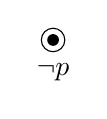
\begin{tikzpicture}
  \draw (0,0) node [desig] {}; % designation
  \draw (0,0) node[world, label=below:{$\neg p$}] (w1) {};
\end{tikzpicture}
with the lever being in the upright position. The action $a_1$ =
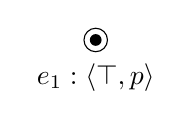
\begin{tikzpicture}
  \draw (0,0) node [desig] {}; % designation
  \draw (0,0) node[world, label=below:{$e_1: \langle \top, p \rangle $}] (w1) {};
\end{tikzpicture}
has the owner $\omega(a_1) = 1$ player 1. Everything is fully observable for the agent. The intuitive  solution should prescribe the action $a_1$ to agent 1, pulling the lever to the right.

A policy $\pi$ for $\Pi = \langle s_0, A, \omega, \gamma \rangle$ is a partial mapping $\pi: S^{gl} \hookrightarrow \mathcal{P}(A)$ so that :
\begin{enumerate}
  \item Applicability\\
    We require actions to be applicable in all states they are assigned to. \\
    for all $a \in S^{gl}, a \in \pi(s): a$ is applicable in $s$.
  \item Uniformity \\
    If the policy $\pi$ presscribes some action $a$ to agent $i$ in state $s$ and agent $i$ cannot distinguish $s$ from some other state $t$, then $\pi$ has to prescribe the same action $a$ for $i$ in $t$ as well. \\
    for all $s,t \in S^{gl} $ such that $ s^{\omega(a)} = t^{\omega(a)}, a \in \pi(s): a \in \pi(t)$
  \item Determinism \\
    We require $\pi$ to be unambiguous for all agents in the sense that in each state $s$ where an agent $i$ is supposed to act according to $\pi$, $\pi$ will always describe the same action for agent $i$.
\end{enumerate}

The properties uniformity and applicability together imply knowledge of preconditions, the property that in each state, an agent who is supposed to preform a particular action must also know that the action is applicable in that state.

We also must allow policies to sometimes prescribe multiple actions of different owners to the same state. This is because the set of indistinguishable states can differ between the agents. To characterize the different outcomes of agents ating according to a common policy, we define the notion of policy executions.

An execution of a policy $\pi$ from a global state $s_0$ is a maximal (finite or infinite) sequence of alternating global states and actions $(s_0, a_1, s_1, a_2, s_2,...)$, such that for all $ m \leq 0$
\begin{enumerate}
  \item $a_{m+1} \in \pi(s_m)$ and
  \item $s_{m+1} \in Globals(s_m \otimes a_{m+1})$
\end{enumerate}
An execution is called successful for a planning task $\Pi = \langle s_0, A, \omega, \gamma \rangle$, if it is a finite execution $(s_0, a_1, s_1,...,a_n, s_n)$ such that $s_n \models \gamma$.

\todo{Do i really need this?}
\extend{übergang} guaranteed to archieve the goal after a finite number of steps. More formally, all of their executions must be successful. As in nondeterministic planning, such policies are called strong (Cimatti et al. 2003) \todo{Quelle?}.

For a planning task $\Pi = \langle s_0, A, \omega, \gamma \rangle$, a policy $\pi$ is called strong if $s_0 \in \text{Dom}(\pi) \cup \{s \in S^{gl} ~|~ s \models \gamma\}$ and for each $s \in \text{Dom}(\pi)$, any extention of $\pi$ from $s$ is successful for $\Pi$. A planning task is called solvable if a strong policy for $\Pi$ exists.
For $ i \in \mathcal{A} $ , we call a policy $i$-strong if it is strong and  $Globals(s_0^i ) \subseteq \text{Dom}(\pi) \cup\{ s \in S^{gl} ~|~ s \models \gamma \}$.

When a policy is i-strong it means that the policy is strong and defined on all the global states that agent $i$ cannot indistinguish between. It follows directly from the definition that any execution of an $i$-strong policy from any of those iniially indistinguishable states will be successful. So if agent $i$ comes up with an $i$-strong policy, agent $i$ knows the policy to be successful.

Sometimes the agent cannot coordinate their plans but rather have to come up with plans indivudually. These plans can differ a lot, the agents could have different reasoning capabilities, have non-uniform knowledge of the initial state and of action outcomes. For this reason we will define a policy profile for a planning task $\Pi$ to be a family $(\pi_i)_{i \in \mathcal{A}}$ where each $\pi_i$ is a policy for $\Pi$. We assume actions to b instantaneous and executed asynchronnously. This leads to the following generalization:

An execution of a policy profile $(\pi_i)_{i \in \mathcal{A}}$ is a maximal (finite or infinite) sequence of alternating global states and actions $(s_0, a_1, s_1,...)$, such that for all $m \leq 0$,
\begin{enumerate}
  \item $a_{m+1} \in \pi_i(s_m)$ where $i=\omega(a_{m+1})$ \\
    Note here the source of nondeterminism as a result from the possiblity of multiple policies prescribing actions for their respective agents.
  \item $s_{m+1} \in Globals(s_m \otimes a_{m+1}) $ \\
    Here the source of nondeterminism is from the possibility of nondeterministic action outcomes.
\end{enumerate}


If all agents have one strong policy in common which all of them follow, then at execution time, the goal is guaranteed to be eventually reached. If, however, each agent acts on its individual strong policy, then the incompatibility of the individual policies may prevent the agents from reaching the goal, even tough each individual policy is strong.

    \chapter{The tokenized approach}\label{chap:approach}

In the example from the beginning, the problem was that both agents $a$ and $b$ wanted to pull the lever to their own goal which results in infinite executions. This problem can be eliminated by introducing a token. With a token, only the player that has the token gets to execute an action. If the agent is done with their own actions, then they can pass the token on to the next player.

There are different ways to model the token. We are going to start with adding an action that lets one agent hand the token to the next agent. Modeling the token in the beginning of the planning task is a little bit different, since there are three ways the token can be introduced to the agents.
%\todo{Du nimmst bisher keine Referenz zum Kapitel davor. Wuerde das bedeuten, dass man das "Token nehmen" und "Token abgeben" als Aktion in den Planungsalgorithmus einfuehren muss. Dann wuerde ich das hier schreiben.}
\begin{enumerate}
  \item ``Table token'' - the token is lying on a table and one of the agents can take the token in the beginning. \\
  The disadvantage is that maybe no agent would take the token.
  \item ``give token'' - in the specification of the planning task it is also specified which agent will have the token in the beginning. \\
  The problem with this introduction is that in every new planning task, this has to be written in the definition of the task. In order for the planning task to be efficient, it should be given to an agent who has found a plan.
  \item ``random token'' - the token is given to a random agent in the beginning. If that agent can not preform any action it can pass the token to a player who can. \\
  One disadvantage would be that an agent who knows nothing and has no action will prevent the planning task from ever reaching a goal state.
\end{enumerate}

There are also two different types of tokens. The first type of token can be easily passed from one agent to the next without any restriction. This token makes sure that no unwanted agent performs an action that could lead to a worse plan than before. the second type of token forces an agent to perform an action before handing the token to the next agent. This type of token makes sure that the token is not just passed between the agents, it makes sure the agents contribute to reaching a goal state.

\section{Infinite executions to finite executions}

We are now going to describe a function that takes a planning task and tokenize that task. The goal with the tokens is that only one player gets to make a move at a time.

Given a planning task $\Pi = \langle s_0, A, \omega, \gamma \rangle $, the function \textit{tokenize} will transform the planning task into a tokenized planning task so that for all $a \in A$:
 if $a = \langle pre, \textit{eff} \rangle$, then
   $tokenize(a) =\langle pre \wedge hasToken_{\omega(a)}, \textit{eff} \rangle$. \\
Further we define an action
    $ giveToken^{ij} = \langle hasToken_i, \neg hasToken_i \wedge hasToken_j \rangle $
    for all $i,j \in \mathcal{A}$ with $i \not = j$. \\
Then $ A^{Token}=\{tokenize(a)|a \in A\} \cup \{giveToken^{ij}|i,j \in \mathcal{A}, i \not = j\}$. \\
Moreover: $\omega^{Token}(tokenize(a))= \omega(a)$ for all $a \in A$,
and $\omega^{Token}(giveToken^{ij}) = i$ for all $i,j \in \mathcal{A}$. \\
With $s_0$ depending on the way the token should be introduced to the token:

\begin{enumerate}
  \item Table Token:
    The first action in this planning task is for one agent to take the token off the table. Here we need a new action that, if no player has the token, one player can take the token.\\
    $takeToken_j=\langle \bigwedge\limits_{i \in \mathcal{A}}
    \neg hasToken_i, hasToken_j \rangle \forall j \in \mathcal{A}$ with $\omega(takeToken_j)=j$. Then the planning task starts with no agent having the token
    \todo{$s_0 \cup \neg hasToken_i$ macht keinen sinn. Was macht der Mengenvereinigungsoperator auf Zuständen und Propositionen?
* Auch in den anderen Fällen muss die Konstruktion vom neuen $s_0$ noch formal verbessert werden. }
    $s_0^{tableToken} = s_0 \cup \neg hasToken_i$.
    $V_{tableToken}(hasToken_i)=\emptyset \qquad \forall i\in \mathcal{A}$\\
    $V_{tableToken}(p)=V(p) \qquad \forall p\in P : p \not = hasToken$

  \item give Token:
    a specified agent to be determined by the specifications of the planning tasks. We can model this by having $s_0^{giveToken}(j)$ have the variable $j$, the agent that is supposed to have the token in the beginning.
     $s_0^{giveToken}(j) = s_0 \cup \{\neg hasToken_i|i \in \mathcal{A} \backslash j\} \cup hasToken_j$

  \item random Token:
    a random agent
    to model this we need to define some other things first.
    $W_{randomToken}=\{w_i|w \in W, i\in \mathcal{A}\}$ \\
    $w^i \sim_{randomToken} v^i \text{ iff } w \sim v \text{ and } i=j$ \\
    $V_{randomToken}(p)=\{w_i|w\in V(p), p \not = hasToken, i\in \mathcal{A}\}$ \\
    $V(randomToken_i)=\{w_i|w \in W\}$ \\
    $W^{randomToken}_d=\{w_i|w\in W_d, i\in \mathcal{A}\}$ \\
    $s_0^{randomToken}=\langle W_{randomToken}, \sim_{randomToken}, V_{randomToken}, W_{randomToken} \rangle$ \\
    The intuition behind this is duplicating the model for each agent. Because then there are multiple designated worlds, this leads to nondeterminism between the worlds.
\end{enumerate}



Then $ \Pi^{\text{Token}} = \langle s_0^{\text{Token}}, A ^{\text{Token}}, \omega ^{\text{Token}}, \gamma \rangle $.

The action $giveToken$ can have different costs. One option would be to have the the action cost nothing, then the overall cost of the plan would not change. The problem with this is it does not prevent the agents from just passing the token around without a goal. The other option is that the action has the cost 1, then the agents will not just pass the token around,, they will prefer to act themselves if it is more or equally efficient than to let someone else act before handing the token to the next agent.

In searching for the optimal plan the search tree can have a smaller width, because the amount of agents that could perform the next action is limited. Therefore the search tree will probably have a deeper depth, because the action handing off the token will also have to be modeled. This could be researched in the future.

%\extend{Lever example with tokens}

Given this formalization, we can now show that we can stop infinite executions from happening in planning tasks by transforming the planning task into a tokenized planning task.

\begin{theorem}
Under the condition of optimal plans one can prevent the appearance of infinite executions in solvable planning tasks with asynchronous execution order with the introduction of a token based execution order.
\end{theorem}


\begin{proof}[proof sketch]
  The execution is finished when an agent that has the token does not want to do anything. \\
  When an agent $i$ that has a plan gets handed the token, that player has three possible actions:
  \begin{enumerate}
    \item to keep the token and execute an action $a$, which will lower the subjective costs of the remaining policy by at least 1 because the next action is an own action.

    \item to give the token to another agent. In order to pass on the token, the agent that has found the plan would have already performed a perspective shift for the next agent in order to check if the next agent could also find that plan and calculated the subjective cost of the remaining plan. The agent that receives the token will only act with respect to a plan that is at least as good as the plan envisioned by agent $i$.


    \item to do nothing. This will stop the execution.

  \end{enumerate}
  Every agent that will get the token in the plan will either decrease the subjective cost of the policy or stop the execution. Because every agent in the execution decreases the subjective cost, the planning task is executable in infinite executions.
\end{proof}


\section{The prevention of deadlocks}

A deadlock for a policy profile $(\pi_i)_{i \in \mathcal{A}}$ is a global state such that:
\begin{enumerate}
  \item $s$ is not a goal state \\
    Something still needs to be done
  \item $s \in \text{Dom}(\pi_i)$ for some $i \in \mathcal{A}$ \\
    Someone wants something to be done
  \item $\omega(a) \neq i$ for all $i \in \mathcal{A}$ and $a \in \pi_i(s)$ \\
    Nothing will be done because of incompatible individual policies
\end{enumerate}

\begin{wrapfigure}{l}{0.2\linewidth}
\centering
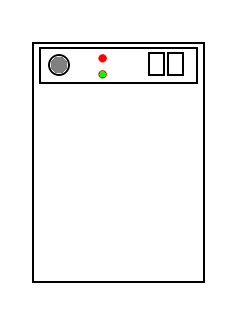
\includegraphics[scale=0.4]{figures/pictures/dishwasher.png}
%\rule{0.9\linewidth}{0.75\linewidth}
%\caption{Dishwasher}
\label{fig:dishwasher}
\end{wrapfigure}


This can be seen in the following example: The two agents from before, Anne and Bill have to empty out the dishwasher. They each have a preference against doing this, since they both spend time (costs) to do this.
In this example you can see that each agent expects the other agent to act, therefore no agent will act.

Let initially, in $s_0$, the dishwasher be full. Agent $1$ has an action $a_1$ and Agent $2$ has an action $a_2$ that can both be applied in $s_0$ and have the effect that has the effect that the dishwasher is empty afterwards. Then the policies $\pi_1 = \{s_0 \xmapsto{a_2} emptyDishwasher \}$ and $\pi_2 = \{s_0 \xmapsto{a_1} emptyDishwasher \}$ are both $i$-strong policies.


Up to this point, the token has given the player that has it the right to perform an action, a right that none of the other players have. But tokens could also force a player to perform an action.

Consider the definition from before with some changes marked in color: \\
Given a planning task $\Pi = \langle s_0, A, \omega, \gamma \rangle $, the function \textit{tokenize-force} will transform the planning task into a tokenized planning task so that for all $a \in A$: \\
 if $a = \langle pre, \textit{eff} \rangle$, then
   $tokenize-force(a) =\langle pre \wedge hasToken_{\omega(a)}, \textit{eff } {\color{UniRed} \wedge doneAction_{\omega(a)}})$ \\
Former we define an Action
    $ giveToken^{ij} = \langle hasToken_i {\color{UniRed}\wedge doneAction_i}, \neg hasToken_i \wedge hasToken_j {\color{UniRed} \wedge \neg doneAction_i} \rangle $
    for all $i,j \in \mathcal{A}$
    \\
Then $ A^{Token}=\{tokenize(a)|a \in A\} \cup \{giveToken^{ij}|i,j \in \mathcal{A}, i \not = j\}
$ \\
Moreover: $\omega^{Token}(tokenize-force(a))= \omega(a)$ for all $a \in A$,
and $\omega^{Token}(giveToken^{ij}) = i$ for all $i,j \in \mathcal{A}$. \\
$s_0^{Token} = s_0 \cup \{\neg hasToken_i|i \in \mathcal{A} \backslash j\} \cup hasToken_j {\color{UniRed} \cup  \{ \neg doneAction_i| i \in \mathcal{A} \}}$ with $j \in \mathcal{A}, |j|=1$\\

With $s_0$ depending on the way the token should be introduced to the token:
\begin{enumerate}
  \item Table Token: The first action in this planning task is for one agent to take the token off the table. Here we need a new action that, if no player has the token, one player can take the token.\\
    $takeToken_j=\langle \bigwedge\limits_{i \in \mathcal{A}}
    \neg hasToken_i, hasToken_j \rangle \forall j \in \mathcal{A}$ with $\omega(takeToken_j)=j$. \\
    Then the planning task starts with no agent having the token or having done an action \\
    $s_0^{tableToken} = s_0 \cup \neg hasToken_i \cup \neg doneAction_i$ \\
    $V_{tableToken}(hasToken_i)=\emptyset \text{ and } V_{tableToken}(doneAction_i)=\emptyset \qquad \forall i\in \mathcal{A}$\\
    $V_{tableToken}(p)=V(p) \qquad \forall p\in P : p \not = hasToken, doneAction$

  \item give Token:
    a specified agent to be determined by the specifications of the planning tasks. We can model this by having $s_0^{giveToken}(j)$ have the variable $j$, the agent that is supposed to have the token in the beginning. \\
     $s_0^{giveToken}(j) = s_0 \cup \{\neg hasToken_i|i \in \mathcal{A} \backslash j\} \cup hasToken_j \cup \{\neg doneAction_i|i \in \mathcal{A}\}$

  \item random Token:
    a random agent
    to model this we need to define some other things first.
    $W_{randomToken}=\{w_i|w \in W, i\in \mathcal{A}\}$ \\
    $w^i \sim_{randomToken} v^i \text{ iff } w \sim v \text{ and } i=j$ \\
    $V_{randomToken}(p)=\{w_i|w\in V(p), p \not = hasToken, i\in \mathcal{A}\}$ \\
    $V(randomToken_i)=\{w_i|w \in W\}$ \\
    $W^{randomToken}_d=\{w_i|w\in W_d, i\in \mathcal{A}\}$ \\
    $s_0^{randomToken}=\langle W_{randomToken}, \sim_{randomToken}, V_{randomToken}, W^{randomToken}_d \rangle$ \\
    \todo{Wie modelliere ich hier doneAction rein?}
    The intuition behind this is duplicating the model for each agent. Because then there are multiple designated worlds, this leads to nondeterminism between the worlds.
\end{enumerate}



Then $ \Pi^{\text{Token}} = \langle s_0^{\text{Token}}, A ^{\text{Token}}, \omega ^{\text{Token}}, \gamma \rangle $.

The changes imply that each agent can only pass on the token when that agent has performed an action.

This new token version also solves the infinite execution problem.

The table token introduction of the token does not prevent deadlocks because in this case, no agent would take the token off the table, which causes a deadlock. Also, the deadlock in this case can only appear in the initial state, in every other state there is always exactly one acting agent.
\todo{Ist das so verständlich?}

\begin{theorem}
  Under the condition of optimal plans one can prevent the appearance of infinite executions in solvable planning tasks with asynchronous execution order with the introduction of a force token based execution order.
\end{theorem}



\begin{proof}[proof sketch]
  The execution is finished when an agent that has the token does not want to do anything. \\
  When an agent $i$ that has a plan gets handed the token, that player first has to perform an action, thereby lowering the subjective cost, and then that player has two possible actions:
  \begin{enumerate}
    \item to keep the token and execute another action, which will lower the subjective costs of the remaining policy profile or
    \item to give the token to another agent. In order to pass on the token, the agent that has found the plan would have already performed a perspective shift for the next agent in order to check if the next agent could also find that plan and calculated the subjective cost of the remaining plan. The agent that receives the token will only act with respect to a plan that is at least as good as the plan envisioned by agent $i$.
  \end{enumerate}
  Every agent that will get the token in the plan will either decrease the subjective cost of the policy or stop the execution. Because every agent in the execution decreases the subjective cost, the planning task is executable in infinite executions.
\end{proof}

\begin{theorem}
Under the condition of optimal plans one can prevent the appearance of deadlocks in planning tasks with asynchronous execution order with the introduction of a force token based execution order with the give token and random token introduction of the token.
\end{theorem}

\begin{proof}[proof sketch]
  Before any player can give away the token, that player has to perform an action. If a player that has found a plan gets the token, that agent first has to do an action. This contradicts the definition of a deadlock.
\end{proof}


\begin{theorem}
  Under the condition of optimal plans one can prevent the appearance of deadlocks in solvable games with asynchronous execution order with the introduction of a token based execution order with the exception of the table token introduction of the token, as long as the giveToken action costs at least 1.
\end{theorem}

\begin{proof}[proof sketch]
  In every agents policy there is an exact sequence of acting agents. Because only one agent can act, the state that some agents are waiting on each other will never appear.
  The one acting agent will then specify the next acting agent, therefore there always will be something done.
\end{proof}


With these results, we do not need to enforce the agents to be eager to avoid deadlock if we use the tokens with costs. We also do not need optimally eager agents to prevent infinite executions if we use tokens. The only problem with tokens is the introduction of the token, especially with the table token. But as long as an agent takes the token off the table, there will be no more deadlocks.

    %\chapter{Experiments}\label{chap:experiments}

\begin{figure}[t]
\begin{centering}
    \subfloat[Some cool graphic]
    {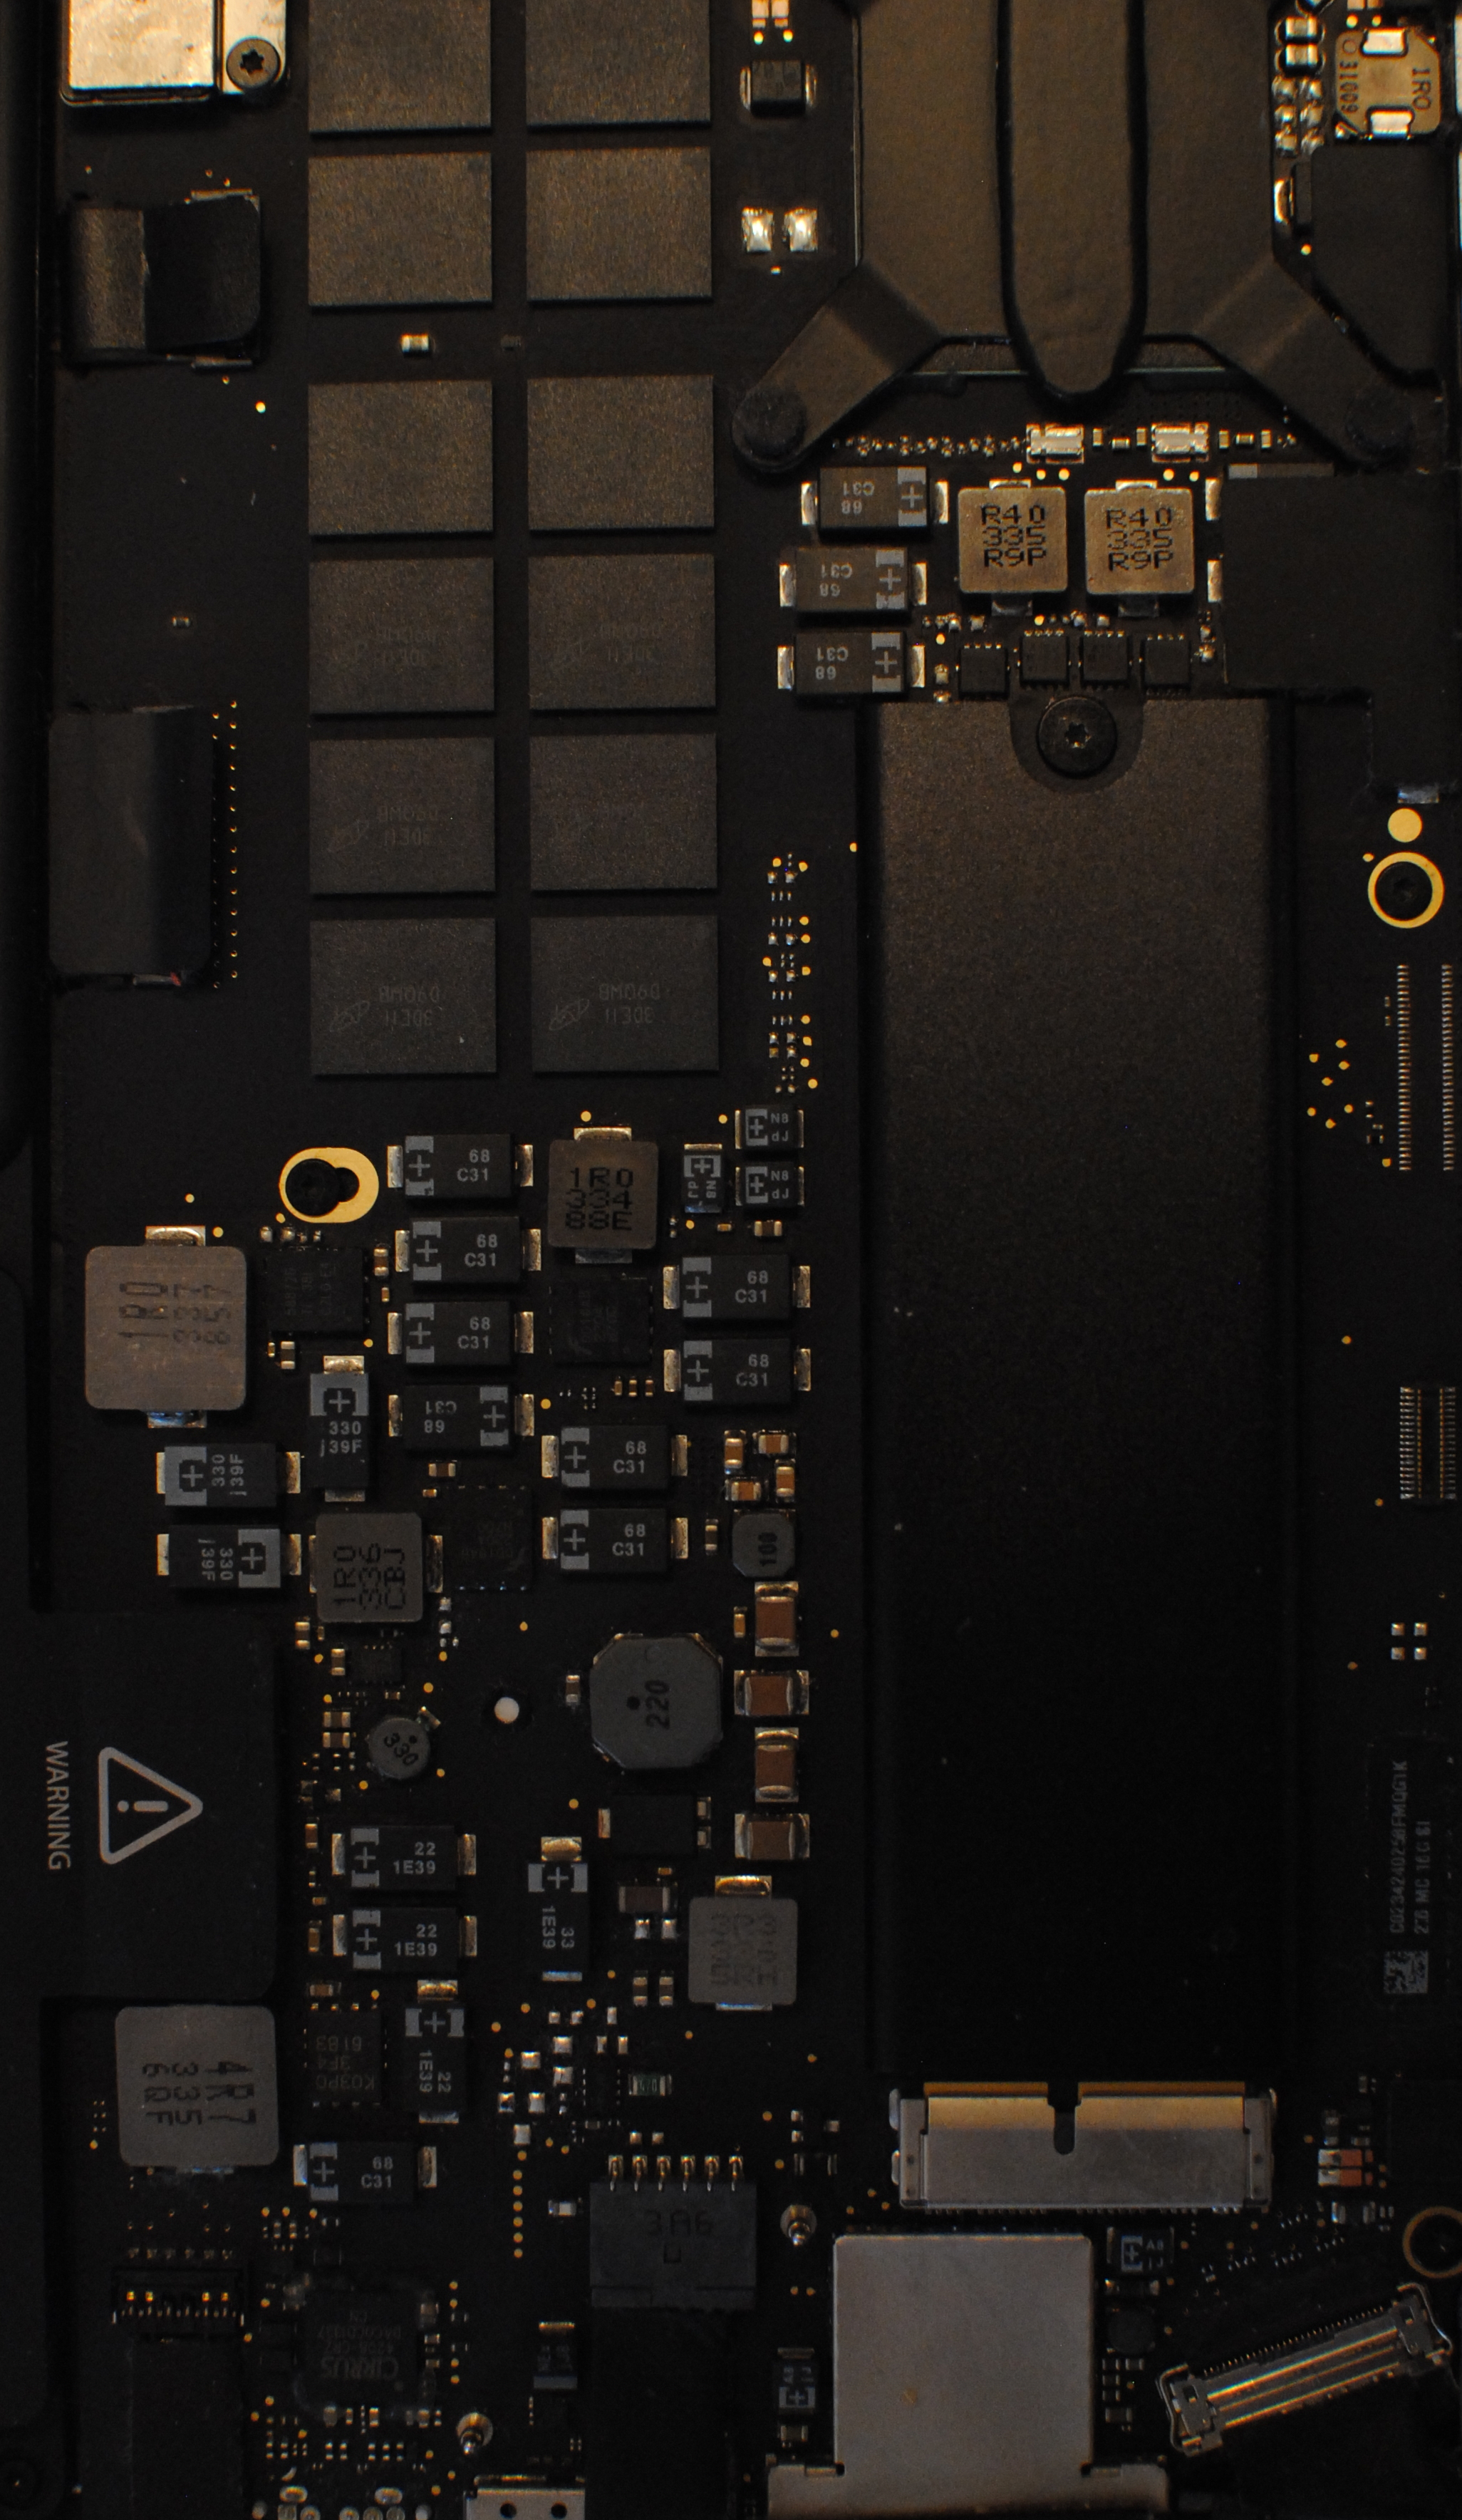
\includegraphics[scale=0.2]{figures/experiments/img.JPG}}

    \subfloat[Some cool related graphic]
    {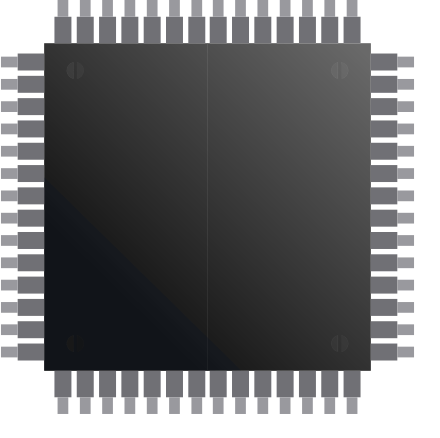
\includegraphics[scale=0.4]{figures/experiments/microcontroller.png}}
    \caption[Caption that appears in the figlist]{\textbf{Caption that appears under the fig} \lipsum[1-1]}
    \label{fig:pcaclasses}
\end{centering}
\end{figure}

\begin{table}[ht]
\centering
% spacing in table
\ra{1.3}
\begin{tabular}{@{}lr@{}}
  \toprule
  Type & Accuracy\\ \midrule
  A    & 82.47 $\pm$ 3.21 \\
  B    & 78.47 $\pm$ 2.43 \\
  C    & 84.30 $\pm$ 2.35 \\
  D    & 86.81 $\pm$ 3.01 \\
  \bottomrule
\end{tabular}

    \caption[Table caption]{\textbf{Table caption.} foo bar...\\}
    \label{tab:accuracy}
\end{table}
    \chapter{Conclusion}\label{chap:conclusion}
    \chapter{Acknowledgments}

First and foremost, I would like to thank...
\begin{itemize}
\item{advisers}
\item{examiner}
\item{person1 for the dataset}
\item{person2 for the great suggestion}
\item{proofreaders}
\end{itemize}

    % If you want a list of your ToDos at the end of the document
    % don't forget to remove before submission!
    % place it somewhere in the document
\chapter*{ToDo Counters}
\newcounter{ct}%
To Dos: \arabic{todos}; \hspace{1em}%
\setcounter{ct}{0}%
\whiledo {\value{ct} < \value{todos}}%
{%
	\stepcounter {ct}%
    \ref{todo \thect}%
	\ifnum\value{ct} = \value{todos}{}\else{, }\fi
}

Parts to extend: \arabic{extends}; \hspace{1em}%
\setcounter{ct}{0}%
\whiledo {\value{ct} < \value{extends}}%
{%
	\stepcounter {ct}%
	\ref{extend \thect}%
	\ifnum\value{ct} = \value{extends}{}\else{, }\fi
}

Draft parts: \arabic{drafts}; \hspace{1em}%
\setcounter{ct}{0}%
\whiledo {\value{ct} < \value{drafts}}%
{%
	\stepcounter {ct}%
	\ref{draft \thect}%
	\ifnum\value{ct} = \value{drafts}{}\else{, }\fi
}


    \bibliographystyle{ieeetr}
    \bibliography{bib/topic1,bib/topic2}
    % bibliography is not in the table of contents per default, add it manually
    % enable the \renewcommand for german header
    % \renewcommand{\bibname}{Literaturverzeichnis}
    \addcontentsline{toc}{chapter}{Bibliography}
    \newpage
    \thispagestyle{empty}
    \mbox{}


\end{document}
